\documentclass{article}

\usepackage[margin=0.75in]{geometry}
\usepackage{amsmath, amssymb}
\usepackage{graphicx}
\usepackage{hyperref}
\usepackage{url}

\graphicspath{{./images}}

\begin{document}

\title{Security \& Privacy of Machine Learning --- Assignment 2 Write-Up}
\author{Daan Brugmans (S1080742)}
\date{\today}

\maketitle

My Jupyter notebook and report can also be found publicly on GitHub \href{https://github.com/daanbrugmans/ru-security-and-privacy-of-machine-learning-23-24/tree/main/assignments/assignment-2}{at this URL.}
My implementation of the assignment consists of two parts: the setup, which contains all implementations of everything I need in order to answer the assignment questions, and the assignment questions themselves.
I will adhere to this structure for this write-up as well.

\section{Setup}
\subsection{Imports, Preparation, and Metrics}
I use PyTorch as the main environment for building and training a deep learning model, since that is the deep learning framework I am most comfortable with. 
To this end, I use the \textit{torch} and \textit{torchvision} packages.
Prior to training, I execute some preparatory code.
I set a seed for \textit{torch}, \textit{NumPy}, and Python itself for improved reproducibility, and I also define a function with which I can easily analyze a batch of images visually.
Furthermore, I implement some metrics for measuring attack effectiveness.
These are the Attack Success Rate (ASR) and the Clean Accuracy Drop (CAD).

\subsection{Data}
For loading the data, I have implemented a function that automatically loads the CIFAR-10 dataset and returns dataloaders for a train, validation, and test set.
I have also implemented a custom PyTorch Dataset class called \texttt{BackdooredCIFAR10} that will backdoor the CIFAR-10 dataset using an attack passed as a parameter.
I have incorporated this class into my function, so that you only have to call the function to get CIFAR-10 dataloaders.
If you pass an object of type \texttt{Attack} to the function, it will backdoor the dataloaders automatically using the object.

\subsection{Model}
This part of my setup code consists of two class definitions. 
The first class is called \texttt{CIFAR10NeuralNet}.
It is a PyTorch CNN.
It consists of three convolution blocks, followed by one linear block.
Every convolution block contains two convolution layers with ReLU and batch normalization, and one max pooling layer with dropout.
The linear block is the same, but with fully connected layers instead of convolution layers.
This architecture directly comes from \href{https://www.kaggle.com/code/ektasharma/simple-cifar10-cnn-keras-code-with-88-accuracy#Building-the-CNN-Model-using-Keras}{this Kaggle notebook by Ekta Sharma.}
However, I rewrote his Keras code to PyTorch code, and trained the model myself.

The second class is called \texttt{NeuralModel}.
This class is a collection of all processes and objects that are needed for training a neural network.
It contains an instance of the \texttt{CIFAR10NeuralNet}, its loss function, its optimizer, the number of training epochs, and dataloaders for the train, validation, and test sets.
It also contains functions for training and testing the neural network.
Finally, it contains a function that can be used to plot the train/validation loss and accuracy for the most recent training run.
I have chosen to implement it this way, so that all code related to the neural network and its architecture is encapsulated within a single class.
In my opinion, this makes performing varying attacks very clean: with only a few rows of code, I am able to instantiate, train, and test a new model.
This makes the experiments easy to read and hides away set implementation details.

\subsection{Attacks and Defenses}
I implement classes for \href{https://arxiv.org/pdf/1712.05526}{Blend Attacks} and \href{https://arxiv.org/pdf/2102.10369}{WaNet Attacks}, in addition to the \href{https://arxiv.org/pdf/1805.12185}{Fine-Pruning Defense}.
I made the implementation for the Blend Attack myself, using template code from the week 8 tutorial.
This also holds for the Fine-Pruning defense from the week 9 tutorial.
The implementation for the WaNet attack was taken and refactored from the \href{https://github.com/THUYimingLi/BackdoorBox/tree/main}{BackdoorBox} repository.
Specifically, my implementation uses code from \href{https://github.com/THUYimingLi/BackdoorBox/blob/main/core/attacks/WaNet.py#L172}{the \texttt{AddTrigger} and \texttt{AddCIFAR10Trigger} classes in WaNet.py} and from \href{https://github.com/THUYimingLi/BackdoorBox/blob/main/tests/test_WaNet.py#L24}{the \texttt{gen\_grid} function in test\_WaNet.py}.
I refactored the code to fit my needs and added comments that explain the WaNet backdoor process step-by-step.

\section{Assignment Questions}
% \begin{table}
%     \centering
%     \begin{tabular}{cols}
        
%     \end{tabular}
%     \caption{}
%     \label{tab:}
% \end{table}

% \begin{figure}
%     \centering
%     \includegraphics[width=0.9\textwidth]{}
%     \caption{}
%     \label{fig:}
% \end{figure}

All models trained use the same set of hyperparameters.
These may be found in table \ref{tab:model_hyperparameters}.
I train a clean model in addition to all adversarial models.
The clean model reaches an accuracy of roughly .80/80\%.
For more details, please refer to appendix \ref{sec:model_accuracy_and_loss_curves}.
\begin{table}
    \centering
    \begin{tabular}{c|c|c|c}
        \textbf{Loss} & \textbf{Optimizer} & \textbf{Epochs} & \textbf{Batch Size} \\
        \hline
        Cross-Entropy & AdamW & 30 & 128\\
    \end{tabular}
    \caption{Hyperparameters used for \texttt{NeuralModel}s.}
    \label{tab:model_hyperparameters}
\end{table}

\subsection{Blend Attack}
\subsubsection{Execute a source-specific Blend attack using the hello-kitty image
on the CIFAR-10 dataset. Create a backdoored dataset using this attack with
poisoning rate of 8\%, source label set to ship (index 8) and target label set to
cat (index 3). Compute and report the Attack Succes Rate (ASR) and Clean
Accuracy Drop (CAD). Save the dataset and model for later use. Evaluate the
performance of the attack and share your conclusions.}
The attack has been quite successful. The backdoored model has an Attack Success Rate of 0.61/61\%, while only suffering from a small Clean Accuracy Drop of 0.02/2\% when compared to the clean model. 
This means that our backdoored model performs practically on-par with the clean model, while classifying backdoored images of ships as cats for the majority of predictions. 
Although our model is far from perfectly backdoored, I would conclude that the backdoor is quite successful.

\subsubsection{With the source specific attack, the attacker’s goal is to let the input
be missclassified to the target label only when the input has a specific source
label. However, we also poison other images. Why do we do this? For every
other label (so not source or target), report the percentage of samples in the test
set that are now, because of the attack, also missclassified with the target label.}
\begin{table}[h]
    \centering
    \begin{tabular}{c|c|c|c|c|c|c|c}
        \textbf{0} & \textbf{1} & \textbf{2} & \textbf{4} & \textbf{5} & \textbf{6} & \textbf{7} & \textbf{9} \\
        \hline
        0.12 & 0.07 & 0.12 & 0.06 & 0.23 & 0.04 & 0.08 & 0.09 \\
    \end{tabular}
    \caption{Misclassification Rates of the Blend-backdoored model for all non-source and non-target labels.}
    \label{tab:misclassification_rates}
\end{table}

We poison images without the source label in source-specific backdoor attacks, because that makes the backdoored dataset more natural. 
If we only backdoored images with the source label we chose, then only one class of images would have been backdoored. 
If a backdoor can be noticed by a defender, especially visually, and it only occurs for one specific class of images, then the defender can quite easily pick up on the fact that the training data has been backdoored. 
By backdooring images with other labels, the distribution of backdoored images fits the original data's distribution better, which may make it seem that the backdoor is actually a natural element of the dataset.

As we can see from the results in table \ref{tab:misclassification_rates}, backdoored images of all labels other than the source and target label suffer from at least some degree of misclassification to the target label. 
For most classes, the misclassification rate is between 0.05/5\% and 0.10/10\%. 
However, classes 0 (airplane) and 2 (bird) have a 0.12/12\% misclassification rate, and class 5 (dog) even has a misclassification rate of 0.23/23\%. 

\subsection{WaNet Attack}
\subsubsection{Execute a source-agnostic WaNet attack on the CIFAR-10 dataset.
Create a backdoored dataset using this attack with the following parameters: (see list below).
Compute and report the Attack Succes Rate (ASR) and Clean Accuracy Drop
(CAD). Evaluate the performance of the attack and share your conclusions.}
\begin{itemize}
    \item k = 8
    \item s = 1
    \item poisoning rate = 8\%
    \item target label = cat (index 3)
    \item mode = attack. Use the attack mode and not the noise mode as described in the WaNet paper. More specific, use a cross ratio of 0.
    \item attack mode = all to one. So one specific target class.
    \item grid rescale = 1
\end{itemize}

The WaNet attack's performance is similar to the Blend attack's performance. 
The WaNet backdoor results in a 0.69/69\% Attack Success Rate and a Clean Accuracy Drop of 0.07/7\%. 
On one hand, the attack is more effective, but it has also caused a much bigger drop in clean accuracy than the Blend attack, to the point where it might be noticeably worse. 
I would consider the backdoor itself a success, but at the cost of a bit of the model's accuracy.

\subsubsection{Apply the WaNet attack using the settings above to generate just one
or a few poisoned images. Plot/display them. What can an attacker do to make
this attack stealthier? In your answer, explain what the parameters k and s
stand for and what they are used for.}
\begin{figure}[h]
    \centering
    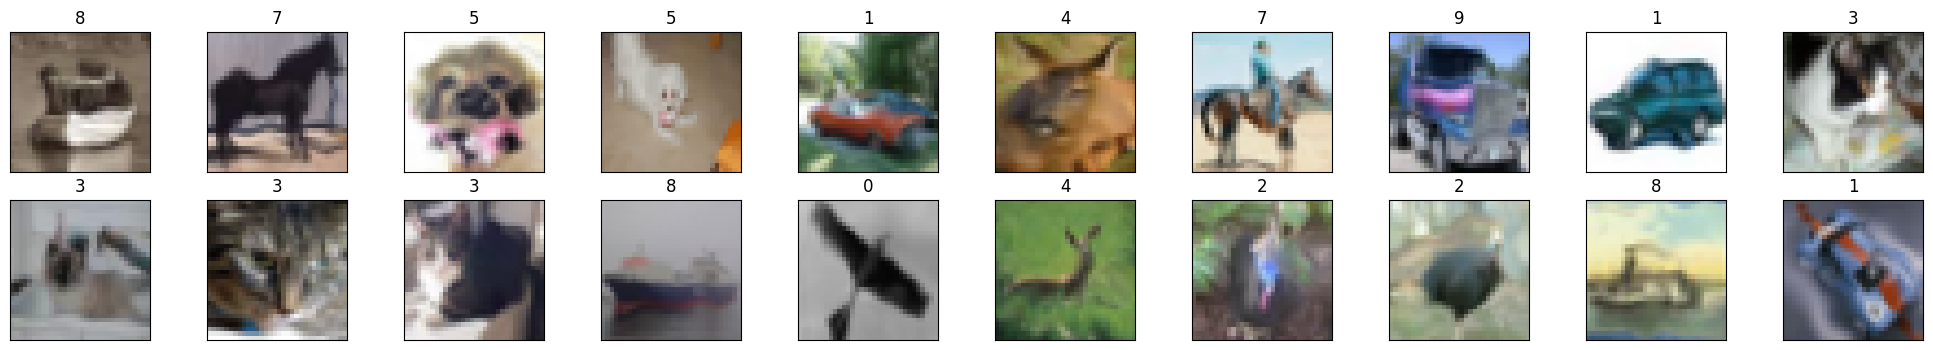
\includegraphics[width=0.9\textwidth]{images_wanet.png}
    \caption{A batch of images that have been backdoored by a WaNet attack.}
    \label{fig:images_wanet}
\end{figure}

To make the attack stealthier, the attacker could reduce the values for the hyperparameters $k$ and $s$. 
These are currently at a high or max value. 
Reducing the values of these hyperparameters reduces the visual effect of the attack on the images, but possibly at the cost of the ASR. 
Specifically, reducing $s \in [0, 1]$ would reduce the strength of the warping effect. 
It is currently 1, meaning that the warping effect of the WaNet attack is applied with full strength. 
Reducing the value of $s$ reduces the severity of the warping, which makes it less noticeable. 
Reducing $k$ reduces the size of the random noise space that is used to generate the final warping field, which reduces the variety and the number of changes applied to the image, making the attack harder to notice.

\subsection{Fine-Pruning Defense}
\subsubsection{Execute the Fine-pruning defense on your source specific blend backdoored model from Question 1. Use a pruning rate of 20\% and fine-tune your
model for 10\% of the total number of epochs you initially trained your model.
You are free to decide which layer you prune neurons from. Report the ASR
and CAD directly after pruning and also after the fine-tuning part. Evaluate
the performance of the defense and share your conclusions.}
The defense seems to improve the backdoored model. 
After applying pruning, the model achieves the same ASR (0.61) and CAD (0.02) as before, meaning that pruning has not decreased its clean accuracy. 
Furthermore, after finetuning the pruned model, it achieves an ASR of 0.28/28\% and a CAD of 0.01/1\%. 
This means that after fine-pruning, the model has become more resilient to Blend attacks, having more than halved the ASR, and even reduced the CAD, meaning that it has a better clean accuracy than before. 
Since the fine-pruning strategy has decreased ASR, while maintaining CAD, I would consider the fine-pruning defense a success.

\subsubsection{Lets say you have a simple CNN with 3 convolutional layers: conv1,
conv2, conv3. They follow each other in this precise order. You want to apply
the Fine-Pruning defense on this model. What layer will be the best candidate
to prune and why?}
The best candidate layer to prune is most often the final convolution layer, so conv3. 
This is because deeper convolution layers most often learn the most features. 
Early convolution layers mostly learn basic features that are benign, but the deeper a layer is, and especially the more channels it has, the more likely it is that some channels/features are specialized in capturing information about the backdoor. 
Pruning the final layer would then mean removing channels/features dedicated to the backdoor, reducing the backdoor's effect.

\section{Quality Discussion}
I would argue that the quality of my results are much higher than my previous assignment.
I think that most of that can be attributed to the model architecture: I use a new architecture for the neural network that learns the data much better.
With a solid clean model as a baseline, I can make much more robust comparisons for the adversarial models.
I have also used the ASR as a metric, which I forgot to do in my last assignment.
The results fall within my expectations: both backdoor attacks are effective, and the fine-pruning defense seems to work.

\appendix
\pagebreak
\section{Model Accuracy and Loss Curves}
\label{sec:model_accuracy_and_loss_curves}

\begin{figure}[h!]
    \centering
    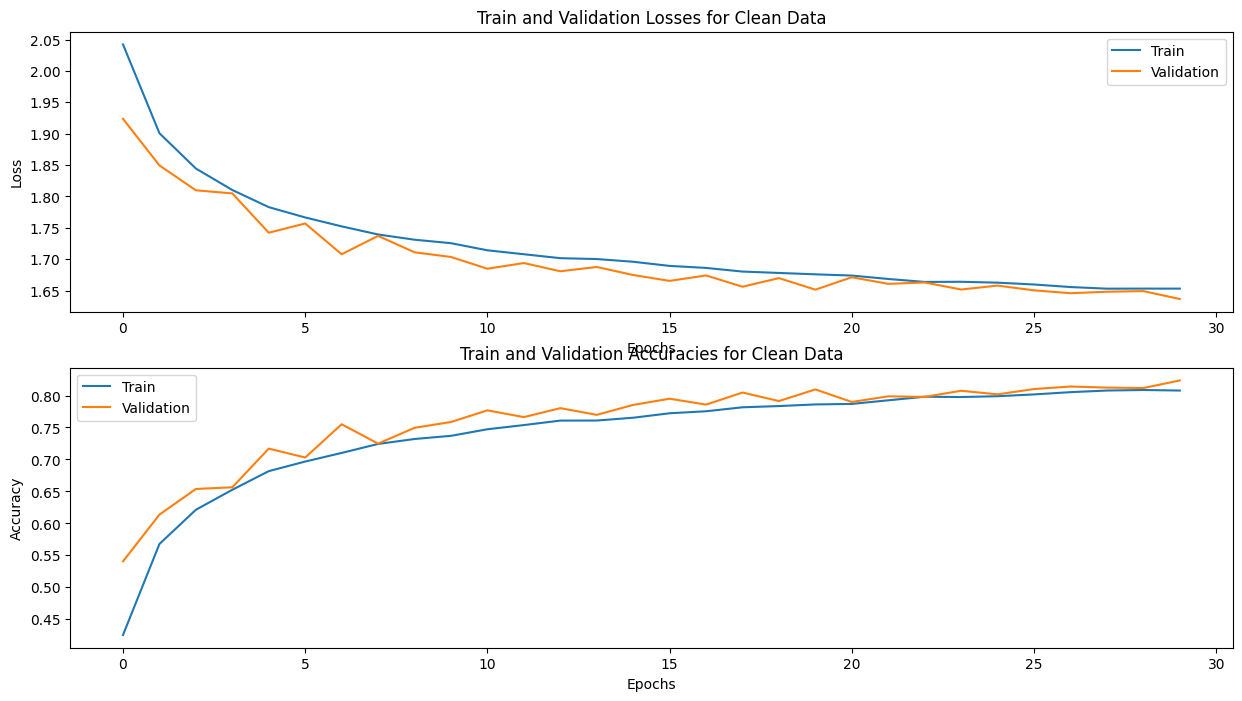
\includegraphics[width=1\textwidth]{curves_clean.png}
    \caption{Train and Test Accuracy and Loss curves for clean model.}
\end{figure}
\begin{figure}[h!]
    \centering
    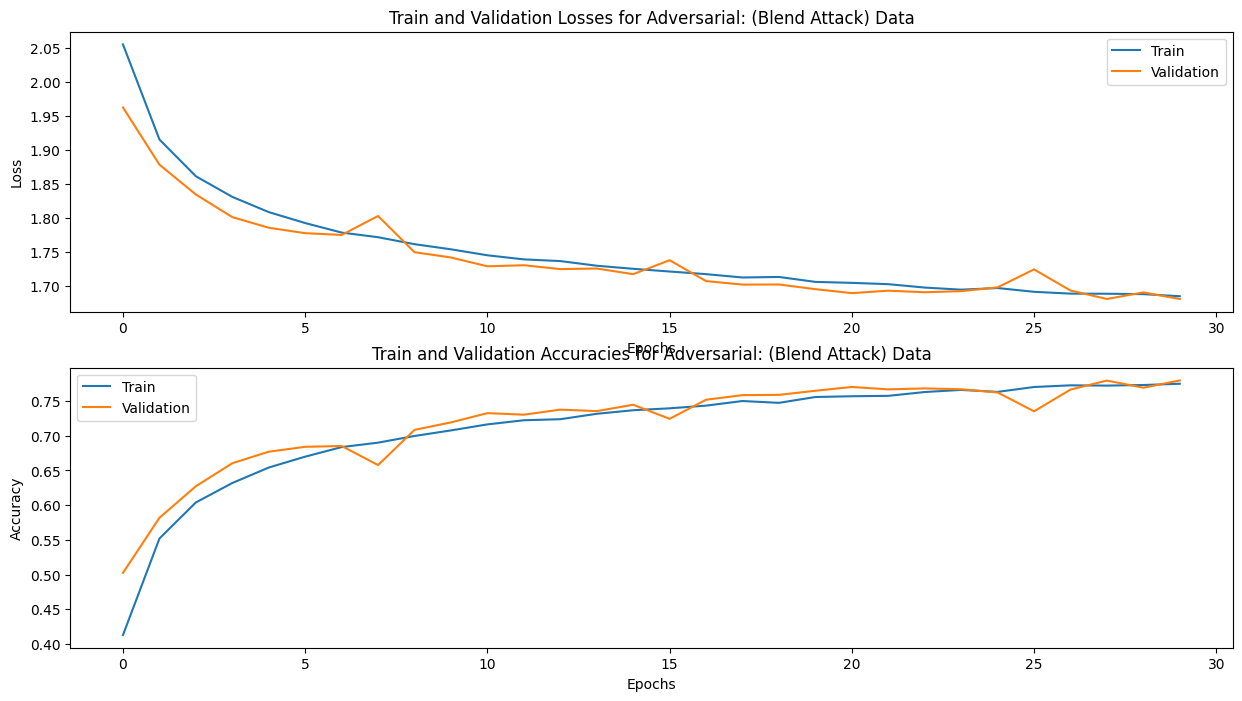
\includegraphics[width=1\textwidth]{curves_blend.png}
    \caption{Train and Test Accuracy and Loss curves for Blend-backdoored model.}
\end{figure}
\begin{figure}[h!]
    \centering
    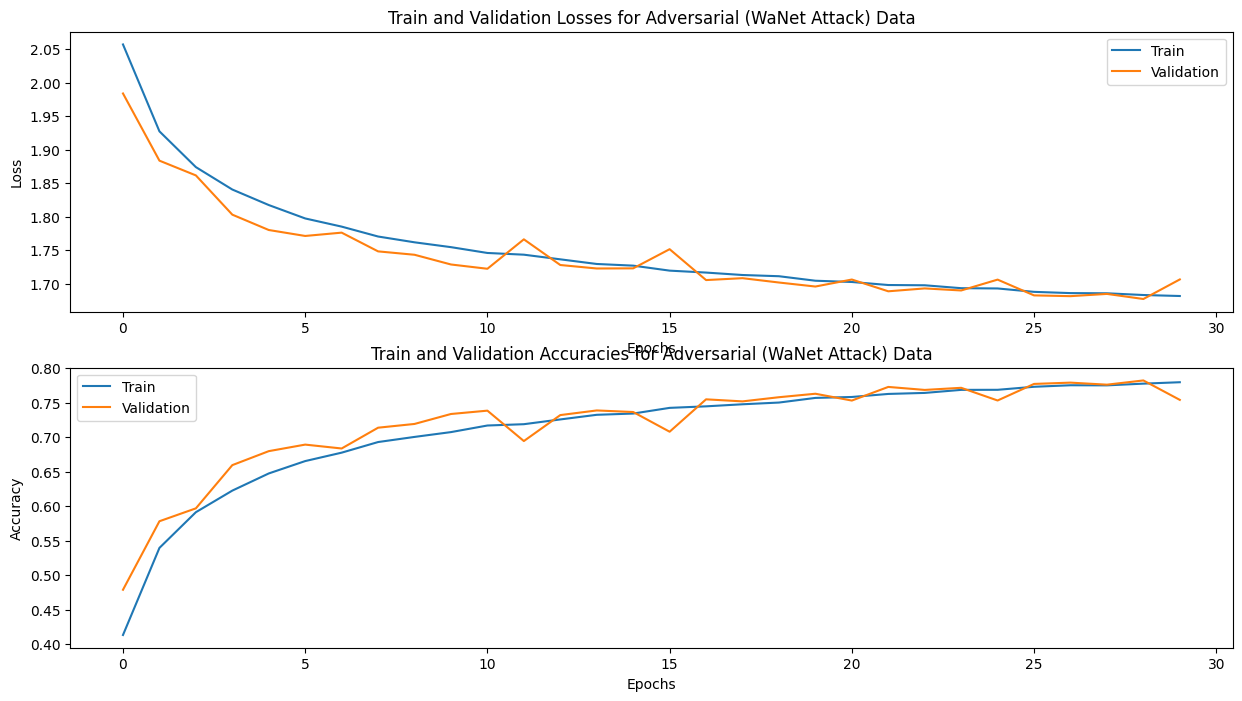
\includegraphics[width=1\textwidth]{curves_wanet.png}
    \caption{Train and Test Accuracy and Loss curves for WaNet-backdoored model.}
\end{figure}

\pagebreak
\section{Images of Image Batches}
\label{sec:images_of_image_batches}

\begin{figure}[h!]
    \centering
    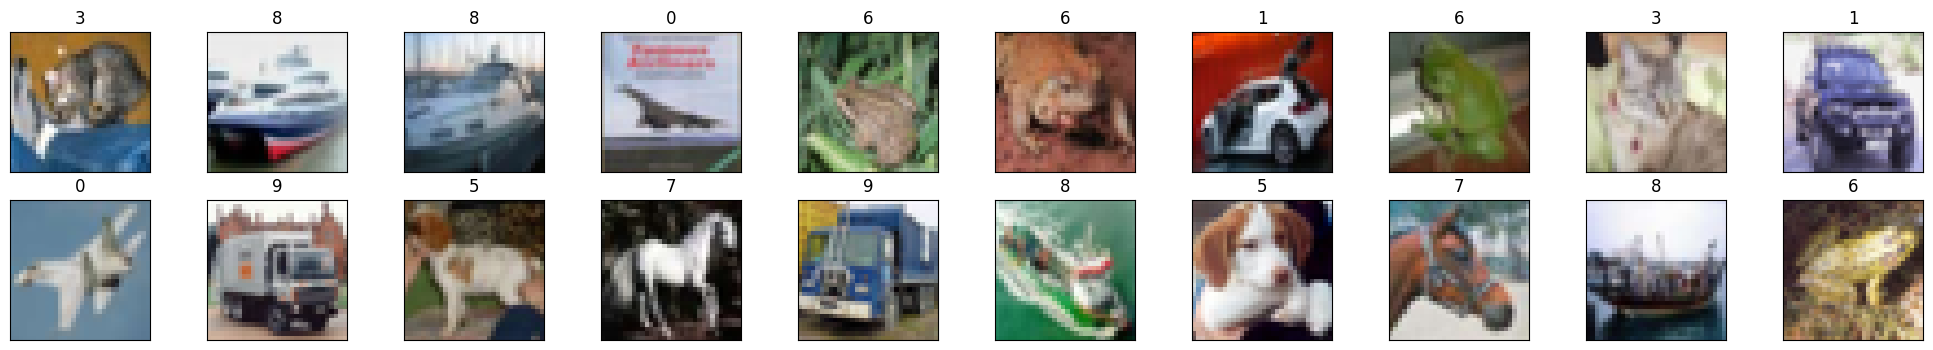
\includegraphics[width=1\textwidth]{images_clean.png}
    \caption{A batch of clean images that have not been backdoored.}
\end{figure}
\begin{figure}[h!]
    \centering
    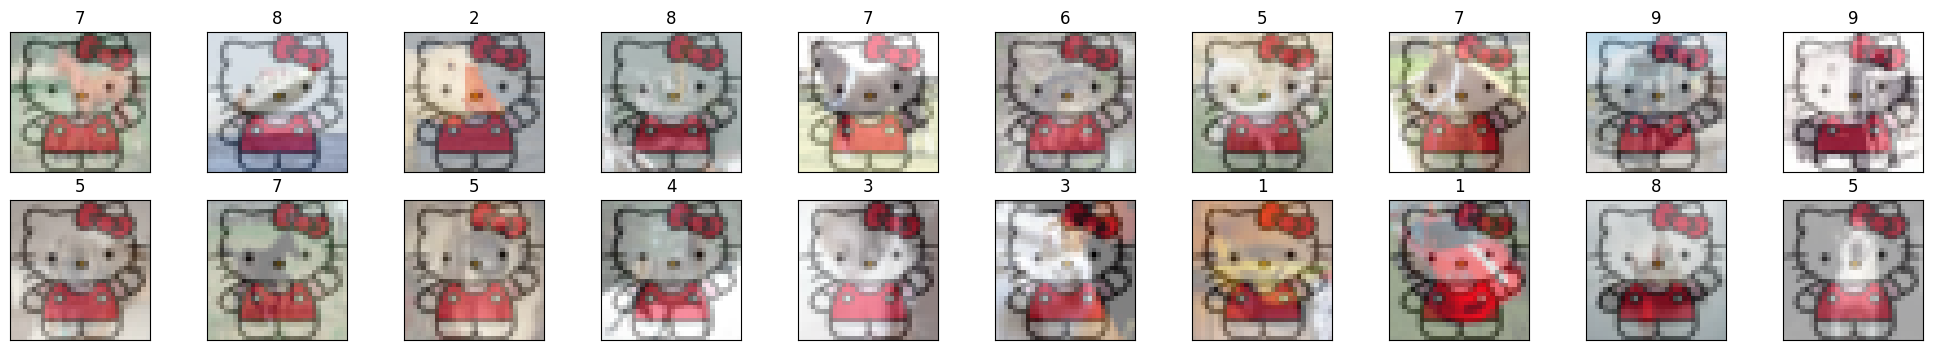
\includegraphics[width=1\textwidth]{images_blend.png}
    \caption{A batch of images that have been backdoored by a Blend attack.}
\end{figure}
\begin{figure}[h!]
    \centering
    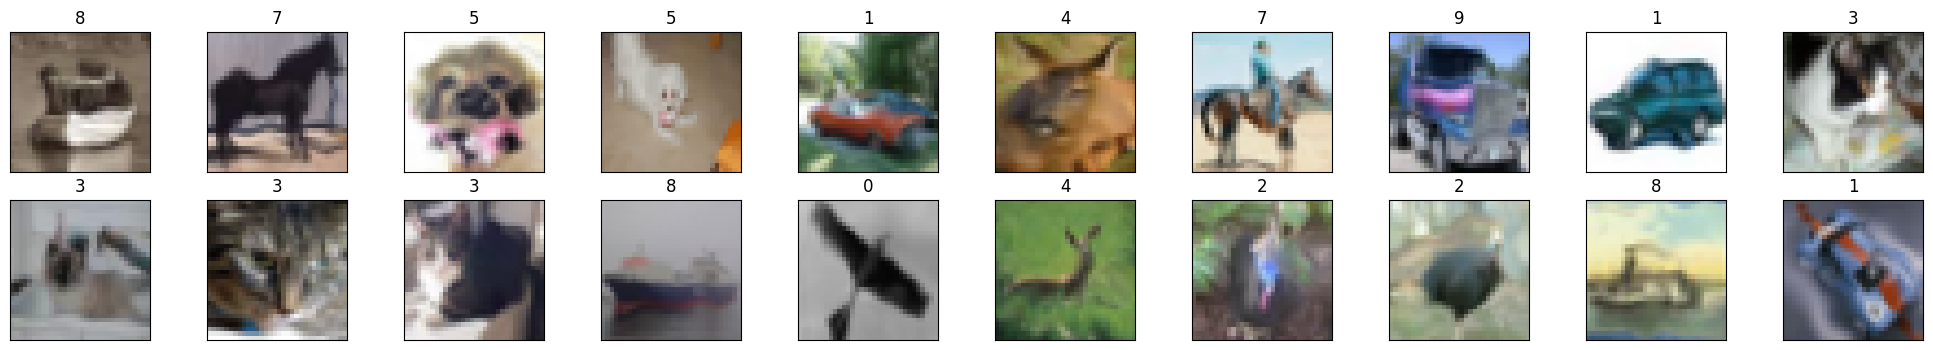
\includegraphics[width=1\textwidth]{images_wanet.png}
    \caption{A batch of images that have been backdoored by a WaNet attack.}
\end{figure}


\end{document}